\documentclass[11pt, oneside]{article}   	% use "amsart" instead of "article" for AMSLaTeX format
\usepackage{geometry}                		% See geometry.pdf to learn the layout options. There are lots.
\geometry{letterpaper}                   		% ... or a4paper or a5paper or ... 
%\geometry{landscape}                		% Activate for rotated page geometry
%\usepackage[parfill]{parskip}    		% Activate to begin paragraphs with an empty line rather than an indent
\usepackage{graphicx}				% Use pdf, png, jpg, or eps§ with pdflatex; use eps in DVI mode
								% TeX will automatically convert eps --> pdf in pdflatex		
\usepackage{amssymb}

\usepackage{dcolumn}
\usepackage[table, svgnames, x11names]{xcolor}

\addtolength{\oddsidemargin}{-.875in}
	\addtolength{\evensidemargin}{-.875in}
	\addtolength{\textwidth}{1.75in}

	\addtolength{\topmargin}{-.875in}
	\addtolength{\textheight}{1.75in}



\newcolumntype{d}[1]{D{.}{.}{#1}}

%SetFonts

%SetFonts


\title{Computational modeling}
\author{Nicolas P. Cottaris}
\date{}							% Activate to display a given date or no date

\begin{document}
\maketitle
\section{ISETBio computational model}
\subsection{Overview}
To connect the measured RGC spatial transfer functions (STF) to the underlying retinal anatomy, a computational model is employed which simulates optical, spectral, spatial, and temporal components of the AO stimulation apparatus, as well as the monkey's optics and cone mosaic structure. The model computes an STF, assuming that cone signals are pooled by the center and surround mechanisms of an RGC according to a difference of Gaussians (DoG) spatial profile model. The parameters of the DoG model and therefore, the actual cone pooling weights, are estimating by minimizing the error between the predicted and measured STFs. A schematic overview of this model is depicted in Figure \ref{fig:ModelOverview}. Various model parameters used to simulate various aspects of the experimental conditions are listed in Table \ref{table:ModelParameters}.

\subsection{AO-delivered stimulus modeling}
The AO-delivered drifting monochromatic sinusoidal gratings used to measured RGC STFs during the experiment, are modeled as temporal sequences of ISETBio spatial spectral radiance scenes, where each scene models a different frame of the drifting stimulus. The spectral profile of the monochromatic beam, the spatial extent and resolution, and the temporal characteristic of the AO display subsystem as are all taken into account in generating these scenes. 

\subsection{Retinal stimulus modeling}
The generated scenes are subsequently passed via a diffraction-limited optical system model which accounts for blur in optical in a perfect AO system and which can also account for additional residual amount blur that may occur in a slightly imperfect AO system, for example due to a slight defocus of the stimulus with respect to the plane of cone inner segments. (Say something more here??). The amount of residual blur in not known a-priori, and it is estimated from the model as described below. 

\subsection{Cone excitation response modeling}
In the next stage, spatiotemporal cone excitation patterns to the employed stimuli are estimated from the computed temporal sequence of retinal spatial spectral irradiance images and an ISETBio model of the monkey's cone mosaic. The ISETBio model of the monkey's cone mosaic is generated using an iterative approach [Cottaris et al] from cone density maps measured during AO imaging. In this stage, retinal irradiance is weighted by each cone's spectral quantal efficiency, and spatially integrated within each cone's inner segment aperture. Assuming that cones are adapted to the mean background irradiance, the computed cone excitation responses are converted to cone contrast responses by first subtracting the excitation to the background stimulus and then dividing by it, separately for each cone. Eye movements are assumed to be zero, since the AO apparatus effectively stabilizes stimuli on the retina.

\subsection{RGC spatial pooling modeling}
Next, the computed spatiotemporal cone contrast responses are integrated over space by spatial pooling kernels which simulate convergence of cones to the center and surround mechanisms of an array of model RGCs. For each model RGC, cone inputs to the center and surround mechanism are are weighted and then pooled over space. The pooling weights are determined by the position of the cone driving the center mechanism, and three free parameters: the gain of the center mechanism, $K_c$, the gain of the surround mechanism, $K_s$, and the characteristic radius of the surround pooling mechanism, $R_s$, with the surround pooling mechanism modeled as a 2D circularly-symmetric Gaussian centered on the cone driving the RF center. Since the retinal location of the recorded RGCs is known only approximately (to lie within the central 40 $\mu m$), we construct many model RGCs, one for each cone within the central 40 $\mu m$ of the model cone mosaic. For each of these model RGCs, the $K_c$, $K_s$, and $R_s$ values are estimated by minimizing the error between the model STF and the measured STF. 

\subsection{Computing model RGC spatial transfer functions}
STF of model RGCs are computed as follows. Following spatial integration of cone signals, the temporal response of a model RGC to a grating stimulus of a particular spatial frequency is fitted with a sinusoidal function whose temporal frequency is set to the temporal frequency of the drifting grating. The amplitude of the fitted sinusoid is taken as the magnitude of the STF at that spatial frequency, and the entire STF is obtained by repeating this procedure for stimuli of the examined spatial frequencies. 

\subsection{Model fitting}
In the final step of the model, a multi-start minimizer procedure is used to find the values of $K_c$, $K_s$, and $R_s$ parameters that minimize the error between the model STF and the measured STF. To minimize the chance of getting stuck to local minima of the error function, the multi-start minimizer is ran 1024 times, and the run resulting in the minimum rms error is used to extract the model parameters. This procedure is repeated for each of the assumed positions of the center driving cone within the central 40 $\mu m$, resulting in a spatial map of rms errors between the model STF and the measured STF.

\subsection{Model validation}
To validate model performance, we use a cross-validation approach, in which we train the model by minimizing the error with respect to the STF measured in one recording session, and assess model performance by quantifying the error with respect to the STF measure at a different (cross-validated) recording session. Model performance is then quantified by averaging the RMS errors across the cross-validated sessions. This approach allows us to evaluate model robustness, and further enables comparison of performance across models with different number of parameters. For example, a model in which the RF center is allowed to pool signals in its RF center from more than one cone, has an extra parameter, the radius of the center, and therefore may fit the measured responses (averaged over all recording sessions0 slightly better than the single cone RF center model. However, by evaluating model performance in cross-validated sessions, we can decide whether the more elaborate model can generalize better than the simpler model, in which case it would indeed be more appropriate, or whether the better fit is due to overfitting some idiosyncracy present in the mean data which does not persist across sessions.

\newpage


\begin{table}% put at top of page if possible 
\centering
\begin{tabular}{|r d{3.3}|}
%\begin{tabular}{|r l|}
\hline
\rowcolor{LightSlateGray!35!Lavender} \multicolumn{2}{|l|}{\textbf{retinal modeling (optics)}} \\
\hline
\mbox{pupil diameter} ($mm$) : & 6.7  \\
\mbox{retinal magnification factor} ($\mu m \times deg^{-1}$) : & 199.26 \\
\hline
\hline
\rowcolor{LightSlateGray!35!Lavender} \multicolumn{2}{|l|}{\textbf{retinal modeling (cone mosaic)}} \\
\hline
\mbox{size} (degs) : & \multicolumn{1}{c|}{1.3 $\times$ 1.3}\\
\mbox{max. density} ($10^3 \mbox{cones} \times mm^{-2}$) : & 270.20\\  
\mbox{cone aperture profile} : & \multicolumn{1}{c|}{\mbox{Gaussian}}\\
\mbox{cone aperture characteristic radius} : & \multicolumn{1}{c|}{0.204 $\times \sqrt{2} \times$
\mbox{i.s. diam.}}\\
\mbox{foveal cone characteristic radius (arc.min.)} : & \multicolumn{1}{c|}{0.17}\\
\mbox{L-cone ratio} : & \multicolumn{1}{c|}{0.48}\\
\mbox{M-cone ratio} : & \multicolumn{1}{c|}{0.48}\\
\mbox{S-cone ratio} : & \multicolumn{1}{c|}{0.04}\\
\hline
\hline
\rowcolor{LightSlateGray!35!Lavender}  \multicolumn{2}{|l|}{\textbf{visual stimulation modeling}} \\
\hline
\mbox{monochromatic stimulation (peak)} ($nm$) : & 561.0  \\
\mbox{monochromatic stimulation (FWHM)} ($nm$) : & 5.0  \\
\mbox{retinal pixel size} ($\mu m$) : & 1.03  \\
\mbox{drift rate} ($Hz$) : & 6.0  \\
\mbox{refresh rate} ($Hz$) : & 25.3  \\
\mbox{spatial extent} ($degs$) : & \multicolumn{1}{c|}{0.7 $\times$ 0.7}\\
\mbox{mean power} ($mW \times cm^2$) : & 1.29  \\
\mbox{contrast} : & 1.0 \\
\hline
\end{tabular}
\caption{Modeling parameters}\label{table:ModelParameters}
\end{table}


\begin{figure}[htbp] %  figure placement: here, top, bottom, or page
   \centering
   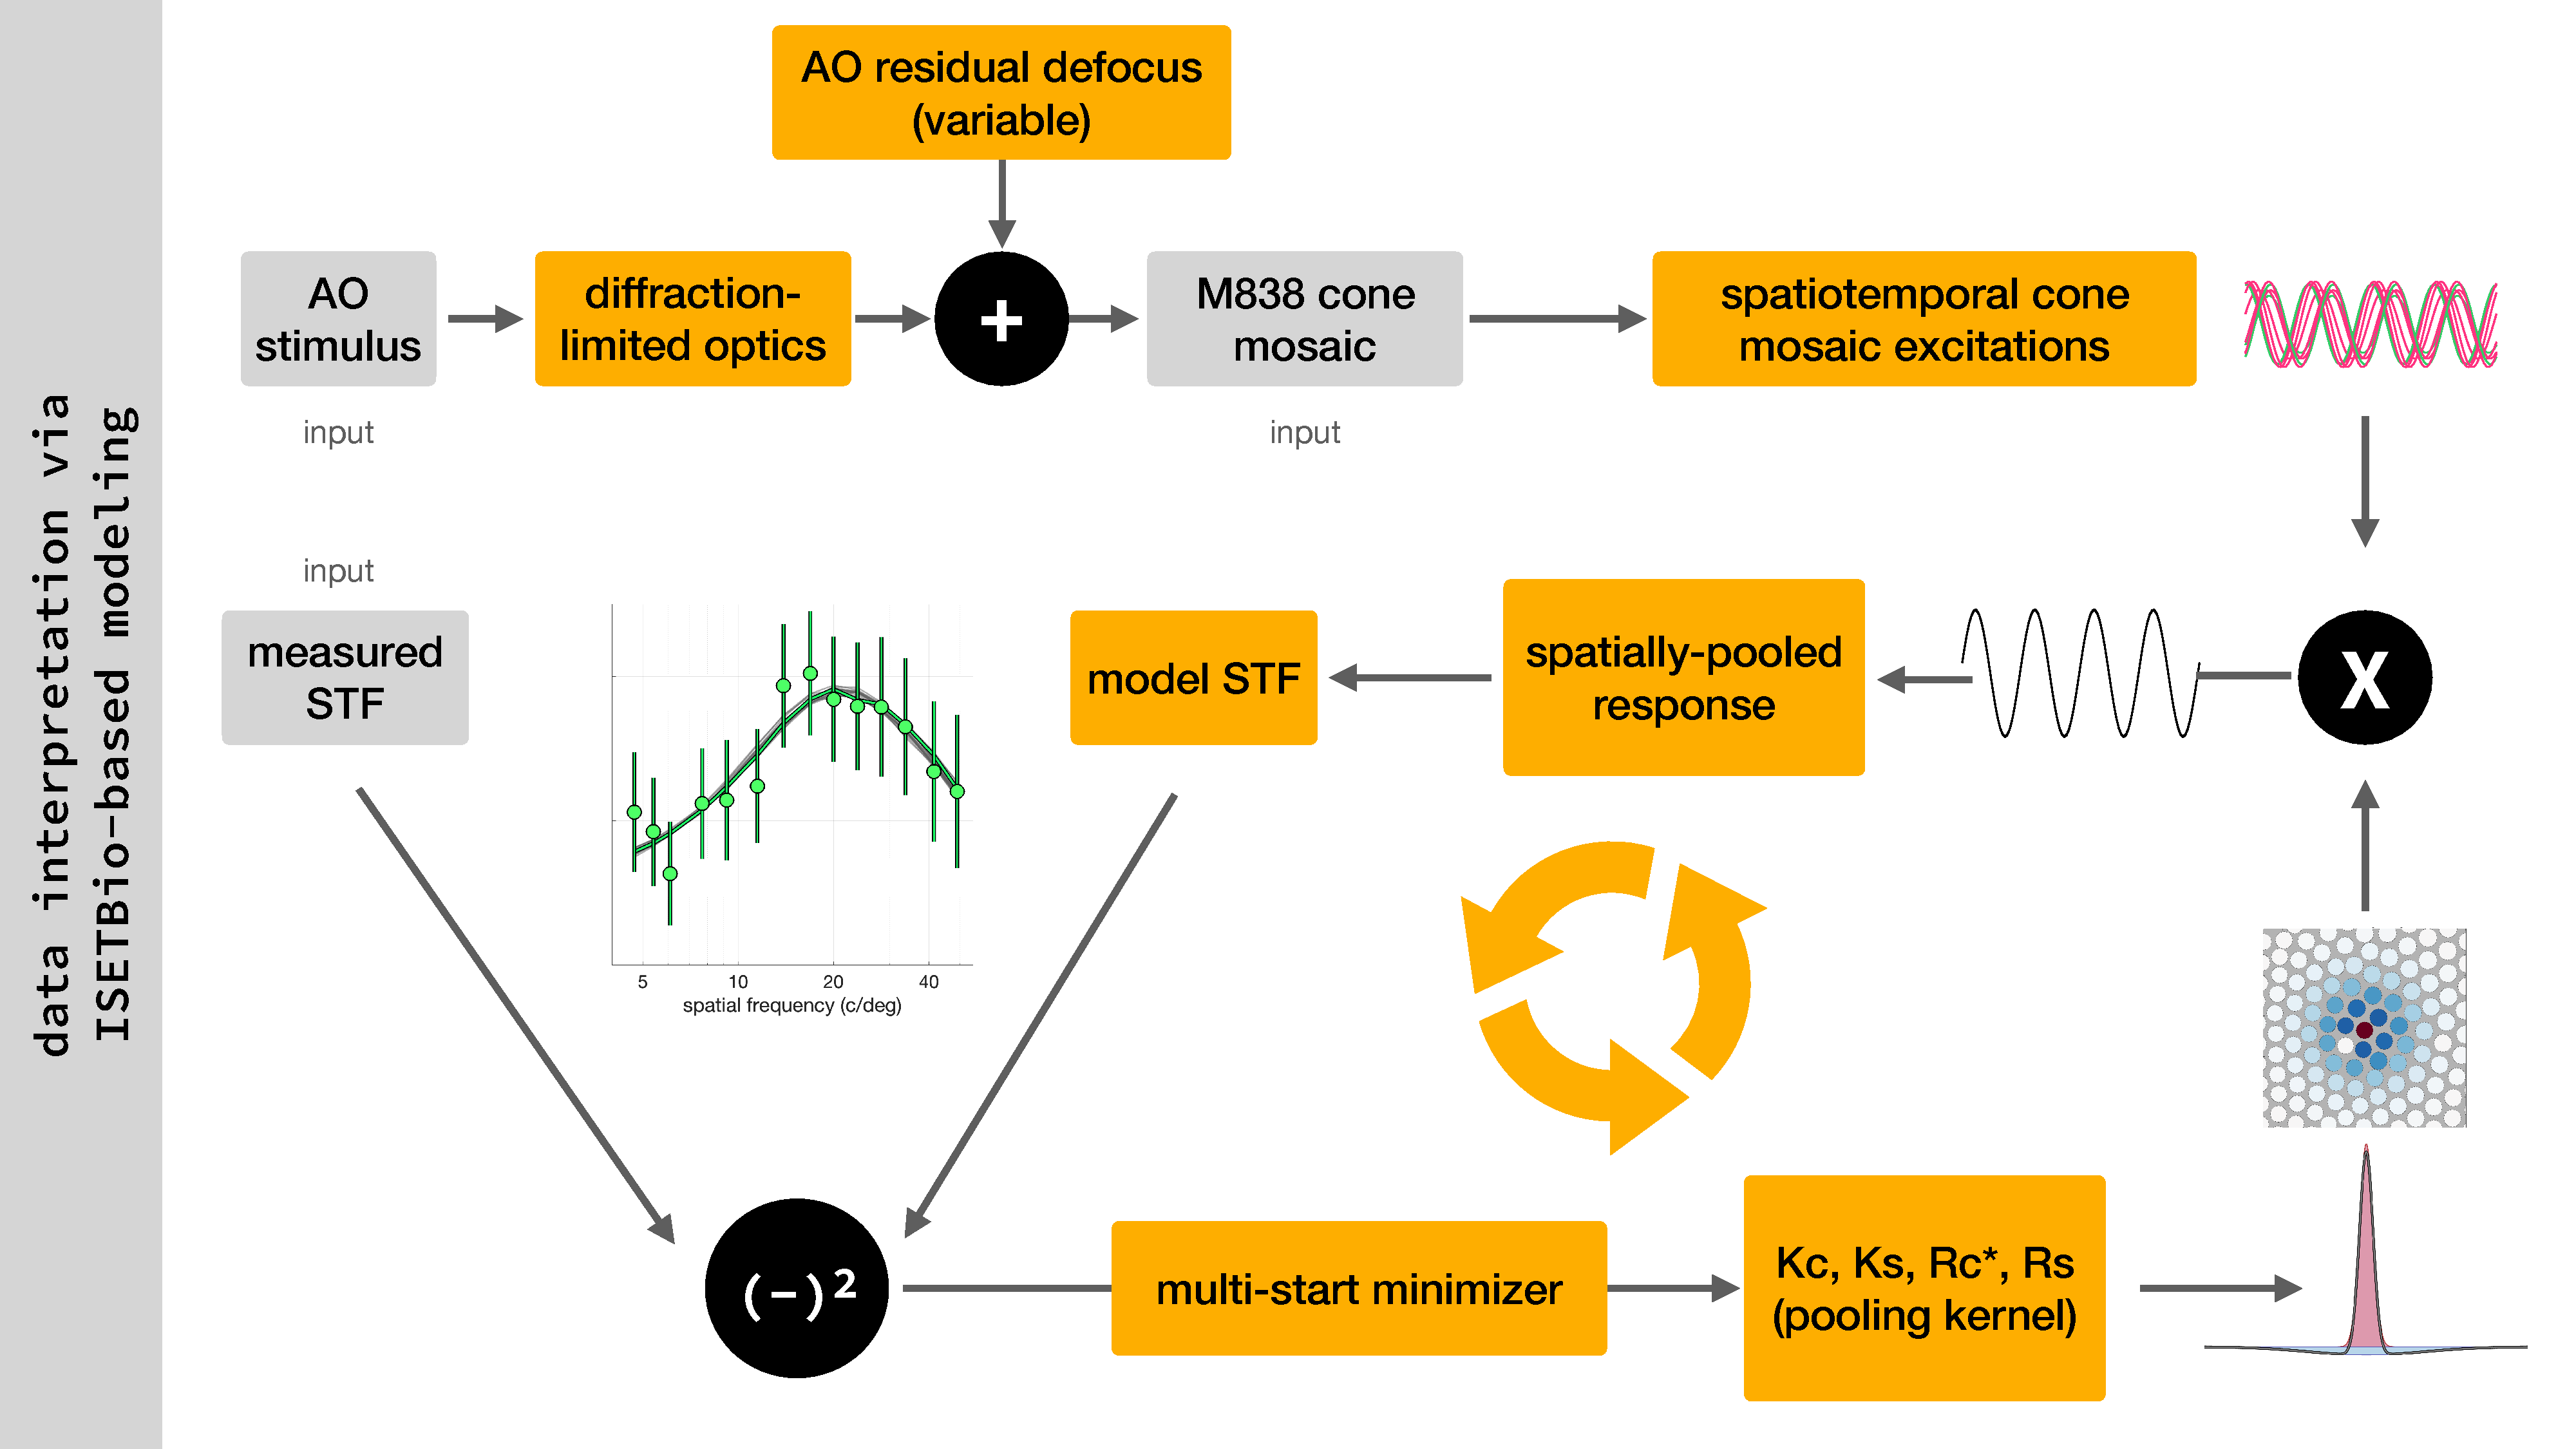
\includegraphics[width=7in]{Figures/ModelOverview.pdf} 
   \caption{Schematic overview of the ISETBio computational model.}
   \label{fig:ModelOverview}
\end{figure}



\end{document}  